\chapter{Introduction}\label{chap:intro}
\textit{While the majority of this chapter was written for the thesis, parts of Sec \ref{sec:astero_intro} were written for \cite{2017North} and have been adapted from the introduction in that work to limit repetition. \textbf{YOU WANT SOMETHING LIKE THIS AT THE START OF EACH SCIENCE CHAPTER TOO, TO SHOW WHAT YOU DID AND ANY ACKNOWLEDGEMENTS OF OTHER PEOPLE}}

\section{Introduction}
The night sky, and the vast emptiness of space has enthralled humanity for all of known history. What is the universe made of? Why do the stars shine? Why do some of them seem to wander across the sky whilst other appear fixed on the celestial sphere? Perhaps most fundamentally, what is our place in the universe and are we alone? It is only with the invention of the telescope that humanity began to unlock the heavens, with the true nature of the universe being far more fascinating than anyone could have imagined. 

In this thesis we will encounter planets orbiting dying stars, and tackle some of the more contentious issues facing exoplanetary astronomy at present. We will use the signature of sound waves trapped inside the stars themselves to uncover their internal and fundamental properties, and discover how the noise signatures of a star can be estimated from its fundamental properties. A topic that will returned to several times throughout this thesis is the use of complementary data, or synergistic usage of the same data to achieve very different results.

Before we start on the main body of the thesis, the contents of each chapter and the main themes within are given in outline first.

Chapter \ref{chap:intro} introduces all the concepts we will explore throughout this thesis, including; methods for detecting exoplanets (and their shortcomings), stellar evolution, asteroseismology and spectroscopy (and their relevant observables). Also covered is how stellar properties are recovered from stellar models used in conjunction with stellar observable parameters. Finally synergies between the separate fields of exoplanets and asteroseismology are possible, and the benefits to both fields. With these concepts introduced we move to the first analysis chapter.

Chapter \ref{chap:reta} immediately introduces a difficult problem in astrophysics, measuring the mass of single stars, particularly evolved stars. If observables are compared to theoretical models to recover the stellar properties, any errors or biases in the stellar model can be compounded by issues in the method used to identify the correct model. Ultimately this can severely bias the recovered stellar mass and all subsequent analysis from this, such as the occurrence rate of planets or the inferred properties of any planets orbiting these stars. In this chapter we focus on the impact of space-based asteroseismology on the recovery of stellar masses for a sample of red giants that have been previously subject to long-term radial velocity observations to detect any planets. 

Chapter \ref{chap:evolvedhosts} keeps us on the theme of evolved stars, incorporating the synergies of asteroseismology and exoplanet science. We look at the potential exoplanet host KOI-6194, believed to be a giant planet on a relatively short period orbit around a red giant star. The unusual binary system KOI-3890 is also studied, a system composed of a red giant star with a low mass dwarf binary component on a highly eccentric orbit. In this system the dwarf star is beginning to tidally distort the primary star, as the primary continues to evolve and expand. This distortion creates a ``heartbeat'' in the lightcurve of the primary star.

In Chapter \ref{chap:spec} we take a break from asteroseismology, and use spectroscopy to investigate another intriguing property of exoplanet hosts. As an ensemble they appear to possess higher levels of elements heavier than helium than non-hosts. Using a homogeneous set of spectroscopic data, we investigate the validity of this theory, when applied to giant stars, with giant planets. 

In Chapter \ref{chap:noise} we use asteroseismic scaling relations, to investigate, and predict the noise levels of evolved stars, and impact of this noise on the detection of exoplanets these evolved giant stars.
Finally the thesis is concluded in Chapter \ref{chap:conc}.


\section{History of stellar and planetary astronomy}
Since prehistoric times, 6 of the planets in the Solar System have been known for ``wandering'' across the sky \ndash with the word planet deriving from the Greek for wanderer. The discovery of Uranus and Neptune (and Pluto) would have to wait until the invention of large telescopes. It was with the introduction of the Copernican model of a heliocentric (centred on the Sun) universe during the Renaissance, that astronomy began to enter the modern realm of scientific thought. This was expanded upon by the work of Galileo, who was the first to observe bodies that did not appear to orbit the Sun, in this case the four major moons of Jupiter, now known as the Galilean moons. 

Galileo can also be credited with the some of the first observations of the Sun through a telescope, and showing that sunspots were features on the ``surface'' of the Sun, rather than orbiting bodies. The apparent motion of the sunspots across the visible face of the Sun also proved that the Sun rotated about an axis, not the static, unchanging body it was considered in antiquity.

\subsection{Existence of planets outside the Solar System}
The first scientific work towards detecting planets around other stars outside the Solar System (hence exoplanet) would have to wait for advanced telescopes to be developed in the mid to late 20th Century, with claimed detections around the nearby M-dwarf Barnard's Star \citep{1963VandK,1969VandK}, which were later refuted \citep{1973Gatewood}. Dedicated surveys using large telescopes and sensitive spectrographs started in the 1980s, with several detections of radial velocity variations consistent with planetary masses \citep{1988Campbell,1989Latham}, (see Sec \ref{sec:doppler}) before the first confirmed detection of a planet around a solar-like star, 51 Pegasi b \citep{51peg}. With the advent of long-term ground and space based surveys to discover exoplanets, thousands of new worlds have now been found \citep{2014Batalha,2014Fischer}. Whilst many of these worlds are unlike any planet seen in the Solar System, they can still be broadly classified into types, based upon fundamental properties. We will introduce the different classes of planets, and methods for observing them, before moving onto stellar physics and asteroseismology.


\section{Types of planets}
\subsection{Types of planets and formation}\label{sec:planetform}
Broadly speaking, a planet's characteristics are entirely determined by the mass gathered during the turbulent era of its formation and its proximity to its host star. If a gravitationally unstable molecular cloud collapses, to form a stellar system, conservation of angular momentum prevents some material from collapsing onto the star. Instead a disk is formed around the forming protostar. It is this material that forms planets, and a means by which planet formation can be considered a natural consequence of star formation.

Since planets require heavy elements to form (carbon, silicon, oxygen, iron etc), it is believed that the very first stars (the not yet observed Population III stars) would have not harboured planets. However once they exploded as supernovae, heavier elements were released into the universe to form the seeds of planets. One of most exciting discoveries of the \Kepler mission was the system Kepler-444 \citep{kep444}, a star that is 11.2 Gyr old, that plays host to 5 small ($\textrm{R}\sim\Re$) planets, thus suggesting planets have been common debris from star formation for most of the history of the universe. 

Below I detail the different types of planets and broad outlines of one possible planet formation theory, namely the core accretion model \citep{1993Lissauer,1996Pollack}. The details are beyond the scope of this work, however the foundation is needed in later chapters when discussing occurrence rates and the properties of the planets around evolved hosts.

\subsection{Terrestrial planets to mini-Neptunes}
In the vicinity of the forming star near the centre of the disc, temperatures are higher and so volatile gases that constituted most of the stellar nebula such as hydrogen and helium cannot condense. This limits the inner planets to forming from the residual materials such as iron and silicates. This material self accumulates into boulder sized objects via electrostatic forces, at which stage gravitational forces begin to be significant. How these boulders form protoplanets is a major stumbling block in planet formation theory %ref
Once protoplanets have formed (Moon-Mars sized objects) the mass of material left in the vicinity of the forming planets determines what happens next. In the case of our Solar System, there was little remaining gas or dust in the inner parts of the system to sustain further planetary growth. Through a series of dynamical interactions, many of the planetary bodies in the inner Solar System collided, or were scattered out of the system entirely, until the 4 planets we know today remained (these interactions most likely leading to the formation of the Moon also). 

In addition to this theory, and tied to the formation of the giant planets, is that the current terrestrial planets in our Solar System may represent a second generation of planets, formed after a so-called ``Grand Tack'' migration inwards and subsequent reversal by Jupiter \citep{2001Masset,2011Walsh,2015Batygin}. The initial migration inwards would capture protoplanets inwards of the young Jupiter in resonances and deposit a significant fraction of the early inner protoplanetary disc into the Sun \ndash either in the form of protoplanets or gas and dust. This theory would explain several oddities of our Solar System; the lack of super-Earth mass planets or Hot Jupiter planets. 

In planetary systems where an outer giant planet does not wander into the inner system, there remains extra material in the vicinity of the young star that allows the rocky planet to accumulate a little more mass, but there is insufficient gas to trigger runaway accretion (see below). This allows for the formation of higher mass terrestrial planets, so-called Super-Earths. At the high mass end of these types of planets ($\textrm{M}\leq10\Me$), small amounts of hydrogen and helium can be gathered from the surrounding nebula, with these planets generally called mini-Neptunes \citep{2009Barnes,2012Mooij}, due to the more extended atmosphere, and lower average density. 


\subsection{Gas/Ice giants}
In the outer Solar System, there remained plenty of dust beyond the so-called ``ice line'', where temperatures drop sufficiently for ices (water, CO$_{2}$, CH$_{4}$ etc) to condense out of the nebula gas \citep{2012Martina,2013Martinb,2016Schlaufman}. This additional material was gathered by the growing planetesimals, until the bodies grow to sufficient size $\geq10\Me$ to directly gather the lightest gases, hydrogen and helium, the primary constituents of the surrounding nebula. This triggers runaway growth, until the gas reservoir in the vicinity of the planet is depleted. Further dynamical interactions during this time can scatter some of these planets to larger orbits, where reduced gas density prevent these planets gathering appreciable gas envelopes. This is a current theory for the formation of Uranus and Neptune \citep{2002Thommes} in our Solar System.

\subsection{Remaining material}
Remaining scattered throughout the early Solar System would have been a large quantity of planetesimals (mountain-sized objects) that would continue to impact all of the planets for a time. This material was either gathered by the planets, ejected from the system (as is believed for the detection of an extrasolar asteroid \citealt{meech2017a}), or migrated into stable orbits. The modern day asteroid belt between Mars and Jupiter, along with the Kuiper Belt and Oort Cloud in the outer Solar System, are believed to be remaining remnants of this material. 

\subsection{Hot Jupiters}
Hot Jupiters are unusual systems, with a giant planet in close proximity to the host star ($P<10$days), in a region of space it is generally believed they cannot form in. The current theory states that giant planets form much like Jupiter, beyond the ice line, and undergo migrations inwards. There are several theories for how the migration occurs \citep{2013Baruteau}. Either the planet interacts with the surrounding gas in the protoplanetary disk, in a fashion to act as a torque on the planet, or planets interact dynamically with large scattering events occurring, sending at least one planet into the inner system, where it will either remain on an eccentric orbit, or tidal forces between the star and planet may circularise the planet's orbit at a smaller semi-major axis \citep{2015Petrovich}. 

These planets are relatively rare with an occurrence rate around 1\% \citep{Johnson2010,Fressin2013}. There is tension between results from different detection methods however, and we will return to this topic in chapters \ref{chap:noise} and \ref{chap:evolvedhosts}. Since such proximity to their stars, they are highly probable to transit (with deep transits) and due to the large radial velocity signals they give due to their higher masses and proximity to the host star, they are over-represented in survey results, giving the illusion they are common. This was particularly the case in the first large exoplanet surveys. 

It is also possible that Hot Jupiters might over time lose their initial atmosphere, leaving only the massive core. CoRoT-7b may be an example of such a planet \citep{2011Leitzinger,2015Ehrenreich}. Two possible subclasses of Hot Jupiters are ``warm Jupiters'' and ``hot Neptunes''.

Warm Jupiters are also Jupiter sized planets, however they exist at higher orbital periods ($10<P\lesssim 50$days), and so incident flux from the host star on the main sequence is lower than for hot Jupiters. Hot Neptunes on the other hand, are giant planets of similar masses to Neptune, on short period orbits. In literature there are further subclasses sometimes discussed, but I shall not be considering them. The evolved host discussed in Chapter \ref{chap:evolvedhosts} would qualify as a warm Jupiter, however due to the evolved state of the host star, the incident flux on the planet is comparable to that incident on hot Jupiters. 

As they age and lose the heat generated and trapped during their formation, hot (and cold) Jupiters shrink in physical radius. It is possible to re-inflate these planets if the incident flux on them increases, for example, as the host stars evolves into a giant star and the luminosity increases dramatically \citep{2015Lopez,2016Grunblatt,2017Grunblatt}. 

\subsection{Exotic planetary systems}\label{sec:exotic_planets}
Whilst the majority of exotic planet systems discussed in this thesis will be giant planets around solar-like main sequence, or red giant stars, more exotic planets and planetary mass objects are possible. I detail below a few particular examples for completeness. These planets are exotic in nature either due to post formation evolution of the system, or due to an unusual formation location.

\subsubsection{Pulsar planets}
Planets orbiting pulsar stars, supernova remnants of high mass ($>8\textrm{M}_{\odot}$) stars have been found to host planets  \citep{1992PulsarPlanet}, and were in fact the first exoplanets to be detected and confirmed. These planets were possibly formed from the supernova debris directly, or from the destruction of a companion star \citep{2011Bailes}.

\subsubsection{Sub-Dwarf B Star planets }
Kepler 70 is an unusual multi-planet exoplanet host. It is a sub-dwarf B star (sdB). These are stars that during the expansion of the star onto the red giant branch somehow lose the outer layers of the star, exposing the contracted core of the star that is still undergoing helium fusion. Few other sdB stars are known to host planets, with V391 Pegasi the first detected sdB host \citep{2007Silvotti}. Whilst sdB stars are in themselves interesting, it is the presence of two extremely short period planets, having orbital periods 5.76 and 8.23 hours, around this star that are of particular note. Reported in \cite{kep70}, it is believed these planets are the cores of giant planets that plunged deep into the red giant envelope of the star, and may have triggered the expulsion of the envelope regions. In this manner planets may directly influence the evolution of their hosts, a theme we will return to later in Chapter \ref{chap:evolvedhosts}.

\subsubsection{Circumbinary planets}
It is also possible to form planets in stable orbits around binary star systems of various mass fractions. \Kepler has discovered several such planets, including planets in the habitable zones of the binary system. One such example is Kepler 16b, a giant planet announced in \cite{kep16}. As might be expected, these systems require interesting dynamics to remain stable over astronomical timescales.

\subsubsection{Free-floating (rogue) planets}
These objects blur the line between stars and planets (see Sec \ref{sec:tobe} for more details). These objects have some similarity to mini-planetary systems, much like the moons of Jupiter or Saturn, scaled. They are also sometimes termed sub brown dwarf stars, depending on the mass of the object, but could also be planets that were ejected from stellar systems due to a dynamic interaction during formation or subsequently. Detecting and characterising these objects is difficult, due to the lack of illumination on the planet for direct imaging, nor the presence of a star to be influenced by the presence of the object. 

\section{To be (a planet) or not to be?}\label{sec:tobe}
Before we move to the body of the thesis, precisely what classifies as a planet should be defined further. There are two main arguments to consider, does the object ever undergo nuclear fusion during its life, and how did it form? 
\subsection{Nuclear burning limit}
Objects below a mass of ${\sim}75\Mj$ (${\sim}0.07Ms$) never achieve the required internal pressure to ignite sustained hydrogen fusion in their cores and so can be considered failed stars, and are called brown dwarfs \citep{1963Kumar}. Below this mass threshold there are various other available fusion pathways that can be sustained for a portion of the object's lifetime \citep{1997Kulkarni}, particularly whilst the brown dwarf is young and still hot from formation.  
At the low mass limit, deuterium burning occurs, with a rule of thumb condition that objects of mass $M>13\Mj$ classified as brown dawrfs \citep{2011Spiegel}.
\subsection{Formation pathway}
The formation of planets is still an area of intense debate, with two leading theories; accretion and direct collapse. The distinction between the lowest mass brown dwarfs and the highest mass planets is a murky region around $M\approx13\Mj$. It is believed that brown dwarfs form in a similar fashion to stars, through the direct gravitational collapse of a gas cloud (in the case of brown dwarfs, the gas cloud fragments and only a small region collapses to form the failed star). Planets are believed to form as a byproduct of this process. As the star forms a disk is formed around the collapsing protostar, due to angular momentum conservation. In this disk dust can accumulate into grains, which self assemble into larger bodies. In this work most of the objects discussed are not particularly close to this mass limit and so are clearly distinguished between being stars and planets. 


\section{Detecting planets}
Since planets are generally much smaller and less massive than the host star, as well as being non-luminous, directly imaging planets against the glare of the host star is typically the limiting factor, though advances in optical systems are expanding the ability to directly image planets \citep{2013Kuzuhara}. 

As such most planets are detected indirectly, through the influence they have on the host star. I will only discuss two highly complementary methods of detecting exoplanets in detail, the transit method utilised by photometric surveys such as \Kepler, and the radial velocity (also known as Doppler wobble) method, utilised by spectroscopic observations, such as used in the discovery of the first exoplanet to be found around a sun-like star 51 Pegasi b \citep{51peg}. Other methods are only briefly discussed after this.
\subsection{Transits}\label{sec:transits}
If a planet passes in front of the star, as viewed from Earth, we see a transit, as the planet blocks a small percentage of the light from the star. The first transiting system discovered was HD 209458 b \citep{2000Charbonneau}. Whether or not the transit is seen from our vantage point is dictated by the solid angle the planet's shadow sweeps out on the sky. Figure \ref{fig:transit_prob} illustrates this.
\begin{figure}[H]
\centering
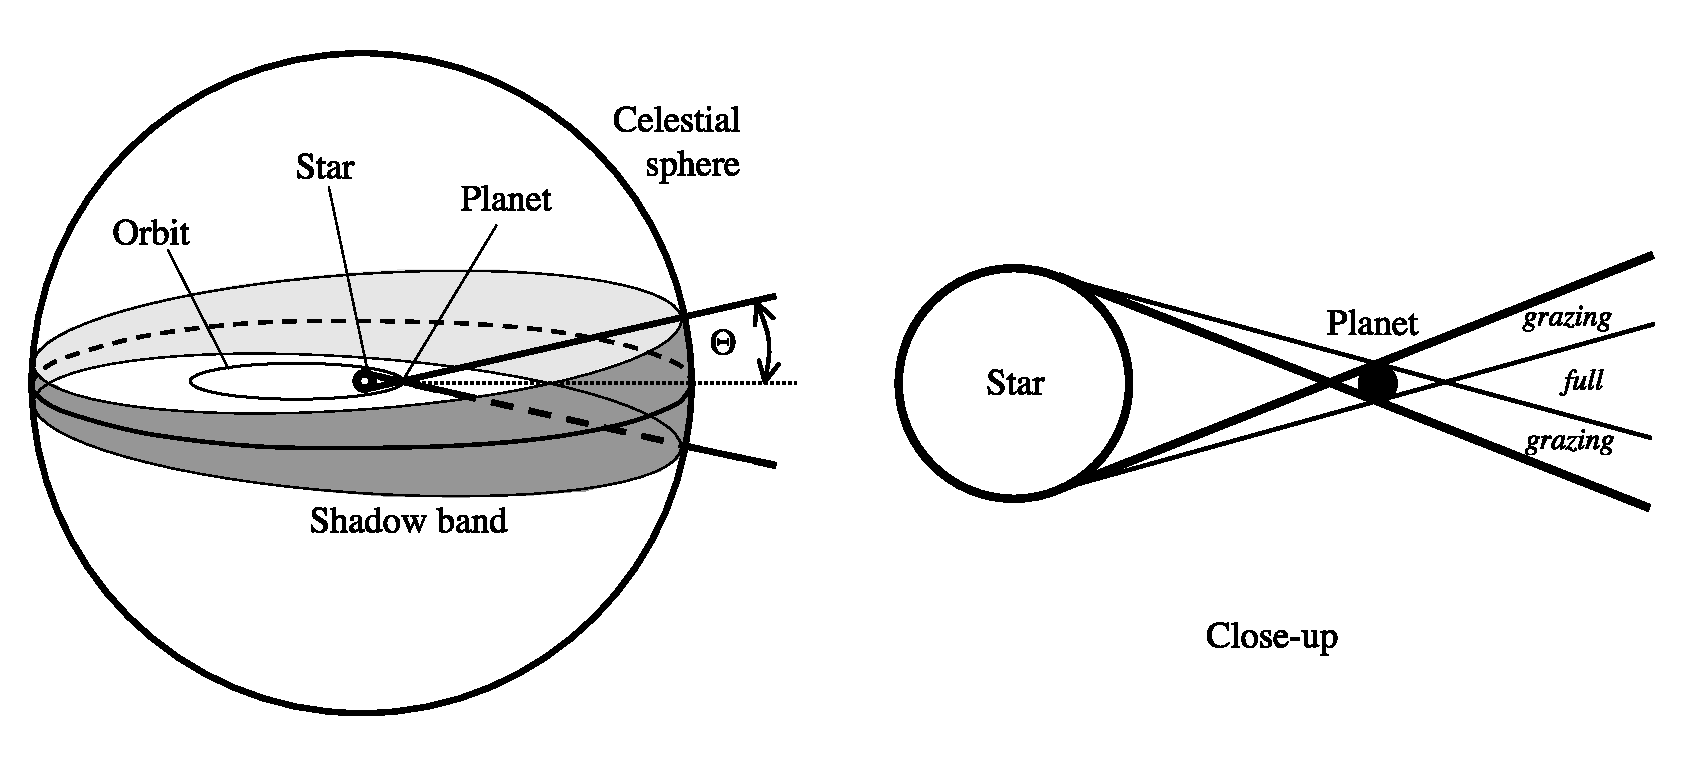
\includegraphics[width=\columnwidth]{probcalc.eps}
\caption{Areas of the sky that observe a transit. As can be seen, for eccentric orbits, the shadow bands covers a greater area of the sky at periastron. The close up on the right represents a flattened version of the geometry, and shows the cases where the transit would be grazing or full. Grazing transits occur within the penumbra, the cone defined by angle $\theta$, with $\sin\theta = (R_{\star} + R_{P})/a$ where $a$ is the semi-major axis of the planet orbit, assuming circular orbits.  Figure from \protect\cite{Winn2010}}
\label{fig:transit_prob}
\end{figure}
As the figure shows, and is intuitively obvious, at periastron \ndash the closest approach of the planet to the star \ndash the shadow band covers the greatest portion of the sky. 

Since a transit is a geometric alignment of host star, planet and observer, it is interesting to investigate the probability of observing a transit around any given star. This has important implications for the minimum size survey required to find a planet in a particular orbit. 

The solid angle of the shadow band in Figure \ref{fig:transit_prob}, assuming circular orbits, is $(2\pi \times 2(R_{P}+R_{\star})/a$, where $a$ is the semi-major axis of the planet orbit. To find the probability the band is along the required line of sight, this solid angle needs dividing by the total solid angle of the sky, $4\pi$, to give the geometric transit probability. If the planet radius is also ignored, and assumed to be negligible compared to the stellar radius, the probability becomes,
\begin{equation}
p_{\textrm{tran}}=\frac{R_{\star}}{a}.
\label{eq:geom}
\end{equation}
\cite{2007Barnes} includes the effect of eccentric planets, and finds that the probability of detection is actually enhanced for eccentric planets, as seen in Eq \ref{eq:geom_ecc} where $e$ is the orbital eccentricity term. 

\begin{equation}
p_{\textrm{tran}}=\frac{R_{\star}}{a(1-e^{2})}.
\label{eq:geom_ecc}
\end{equation}

In the case of an Earth-like transiting system, the geometric probability of detection is 0.46\%, which if inverted provides the average minimum number of systems needing to be observed to find a Earth like transit, 217 systems with solar-like stars, assuming all observed stars have an Earth-like planet on an Earth-like orbit. Obviously this is a simplistic argument, with every corrective factor included (such as true occurrence rate of Earth analog systems) increasing the number of systems required. Eq \ref{eq:geom} also demonstrates an underlying bias in transit searches, i.e. for a given stellar radius, one is biased towards detecting close in planets as they have a higher probability of transiting.

Where on the star the planet appears to cross is called the impact parameter of the planet. It is defined by the angle of planet's orbit observed from Earth, relative to the plane of the sky (see Figure \ref{fig:trandiag}). The exoplanet convention is to define the plane of sky to be $0^\circ$ whilst orbits that lie ``edge-on" as seen from Earth are at an inclination of $90^\circ$. The relation of inclination to impact parameters can be considered by how closely the transit band intercepts the line of sight, i.e. 
\begin{equation}
b\approx\frac{a\cos{i}}{R_{\star}}
\label{eq:impact}
\end{equation}
where $b$ is the impact parameter and is defined between 0 and 1, with $b=0$ corresponding to a $90^\circ$ inclination transit. The impact parameter is primarily of interest in terms of validation of a planet, since high impact planets that transit close to the limb of the star are more likely to be false positives, most likely a misidentified eclipsing binary. 

\begin{figure}[H]
\centering
	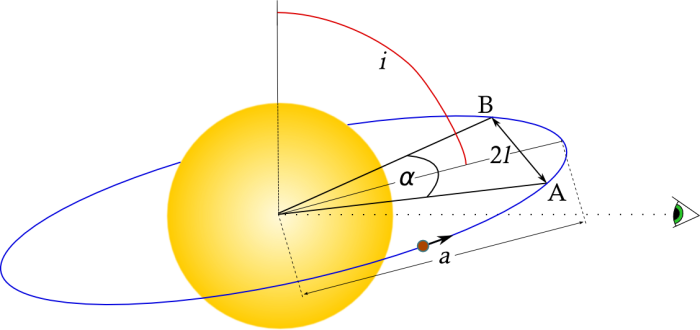
\includegraphics[width=0.7\columnwidth]{general_transit}
    \caption{General geometry of a transit. $i$ is the inclination of the planet relative to the plane of the sky. Therefore most transits are observed around $i=90^o$. During a transit the planet passes through angle $\alpha$, and for a small angle approximation, the chord and arc length between points A and B are considered the same.}
    \label{fig:trandiag}
\end{figure}

It can be easily shown that the fraction of the star's light blocked by the planet ($\frac{\Delta F}{F}$, typically denoted as $\delta$) is proportional to the ratio of the areas of star and planet \citep{Winn2010},
\begin{equation}
\delta \approx \left(\frac{R_{P}}{R_{\star}}\right)^{2},
\label{eq:tran_dep}
\end{equation}
where $R_{P}$ and $R_{S}$ are the planetary and stellar radii respectively. This relation is only approximate due to the star not being a uniformly illuminated body. The is known as limb darkening (see below). This also assumes that the planet is neither emitting, nor reflecting any light (an assumption that is typically valid during transit). In the case that the transiting body does possess intrinsic luminosity (e.g. a binary star system), the equation becomes, 
\begin{equation}
\delta \approx \left(\frac{R_{P}}{R_{\star}}\right)^{2}\left(1-\frac{I_{P}}{I_{\star}}\right),
\label{eq:tran_dep_I}
\end{equation}

Figures \ref{fig:tran_detrend} and \ref{fig:bls_phase} illustrate the transit detection process. The upper panel shows the raw lightcurve of Kepler-423, for 3 quarters of long cadence data (${\sim}30$min integrations). The lower panel shows the lightcurve detrended and normalised around zero, such that transits register as periods of negative flux. 
\begin{figure}[H]
\centering
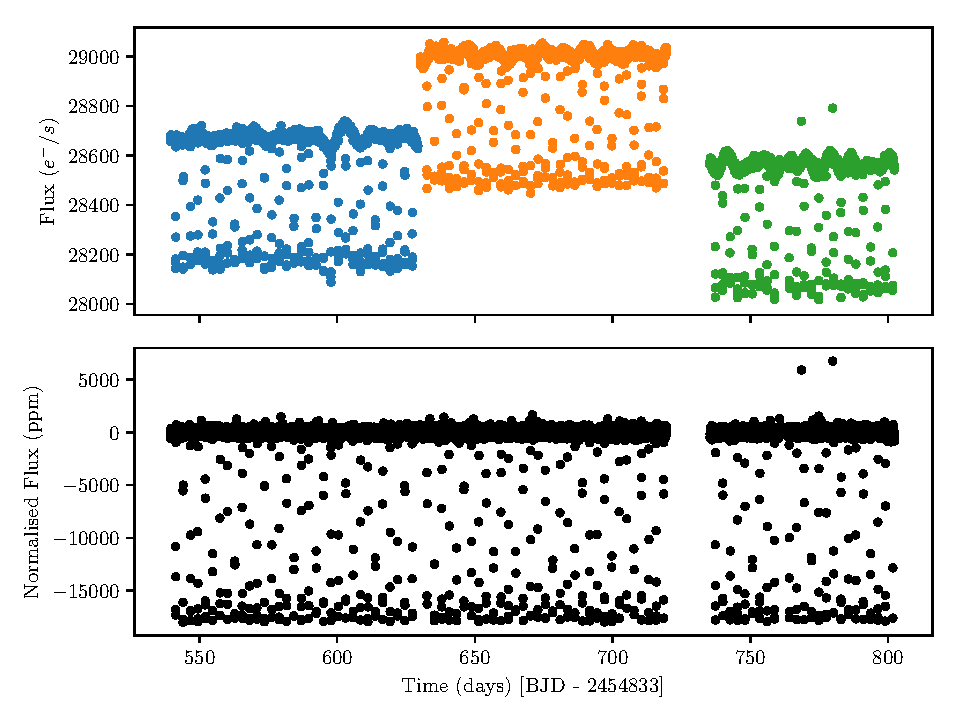
\includegraphics[width=0.75\columnwidth]{Kep_423_tran_detrend.pdf}
\caption{Upper: Kepler-423, raw lightcurve for 3 quarters of long cadence-${\sim}$30 minute integrations, showing a clear transit signature. Lower: detrended lightcurve normalised to zero flux.}
\label{fig:tran_detrend}
\end{figure}
One of the main issues in finding the planets is being able to efficient search the lightcurve for a small periodic signal caused by transits, without being thrown off by other signals. Whilst Figure \ref{fig:tran_detrend} has been chosen to be detectable by eye, normally the method is automated, where efficient search algorithms are required. One method astronomers use is called the ``box least-squares'' (BLS) method \citep{BLS}, that describes the transit as either an inverted top hat function, or a trapezoid, and then rapidly searches for various widths, depths and periodicities of that shape in the lightcurve. 
Figure \ref{fig:bls_phase} shows the result of search a BLS pipeline. The upper panel shows the strength of a signal at a given period. The lower plot is the lightcurve phase-folded on the best period the BLS search found. As expected it stacks the transits on top of each other. The upper panel also shows that such a search algorithm can be disrupted by aliases of the true period. 
\begin{figure}[H]
\centering

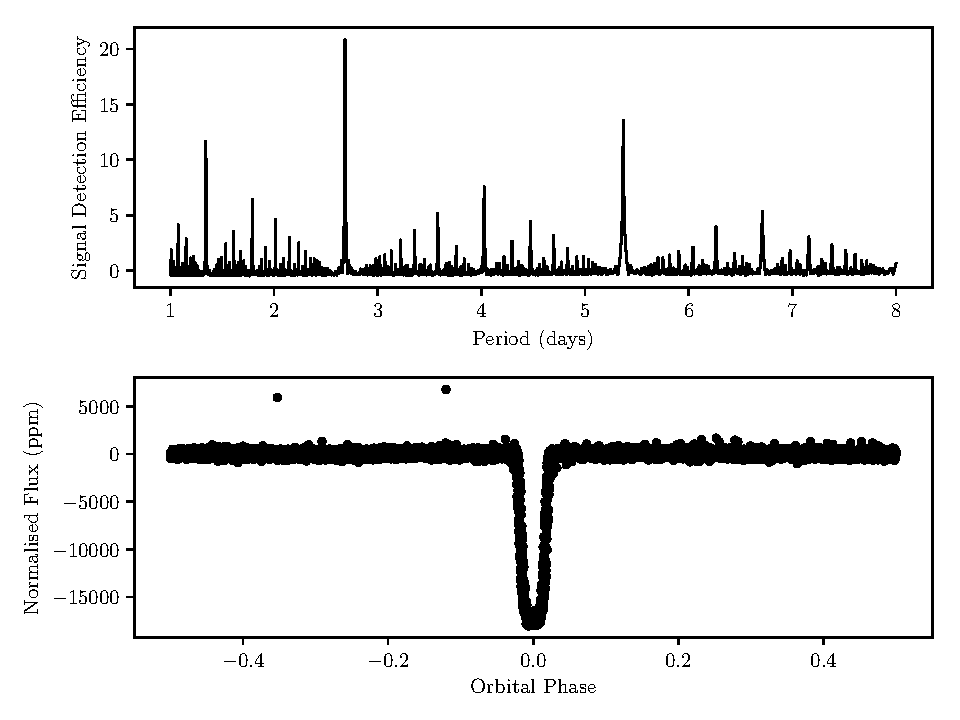
\includegraphics[width=0.75\columnwidth]{Kep_423_BLS_Detection.pdf}
\caption{BLS search for a transit. A strong signal is found at ${\sim}2.75$days, and at the harmonic of that at $5.5$days. The lower panel shows the lightcurve of Kepler-423 folded on the detected period, with the transit clearly visible.}
\label{fig:bls_phase}
\end{figure}
The lower panel of Figure \ref{fig:bls_phase} also illustrates the impact of limb darkening on the shape of a transit. Photons emitted from near the limb (edge) of the star, in order to be detected on Earth, have to travel through more of the star's atmosphere to reach Earth, compared to those emitted from the centre of the disk. Since photons can be scattered in the stellar atmosphere, only those emitted higher in the atmosphere are able to escape to reach our detectors, so we cannot see to the same optical depth on the limb of the star as the centre. Therefore the ``surface'' of star is not a constant radius. The photons detected from the centre of the star are from greater depth inside the star, and subsequently from regions of higher temperature. This has the effect of the star appearing brighter in the centre of the disk. This can clearly be seen in an image of the Sun in Figure \ref{fig:limb}.
\begin{figure}[H]
\centering

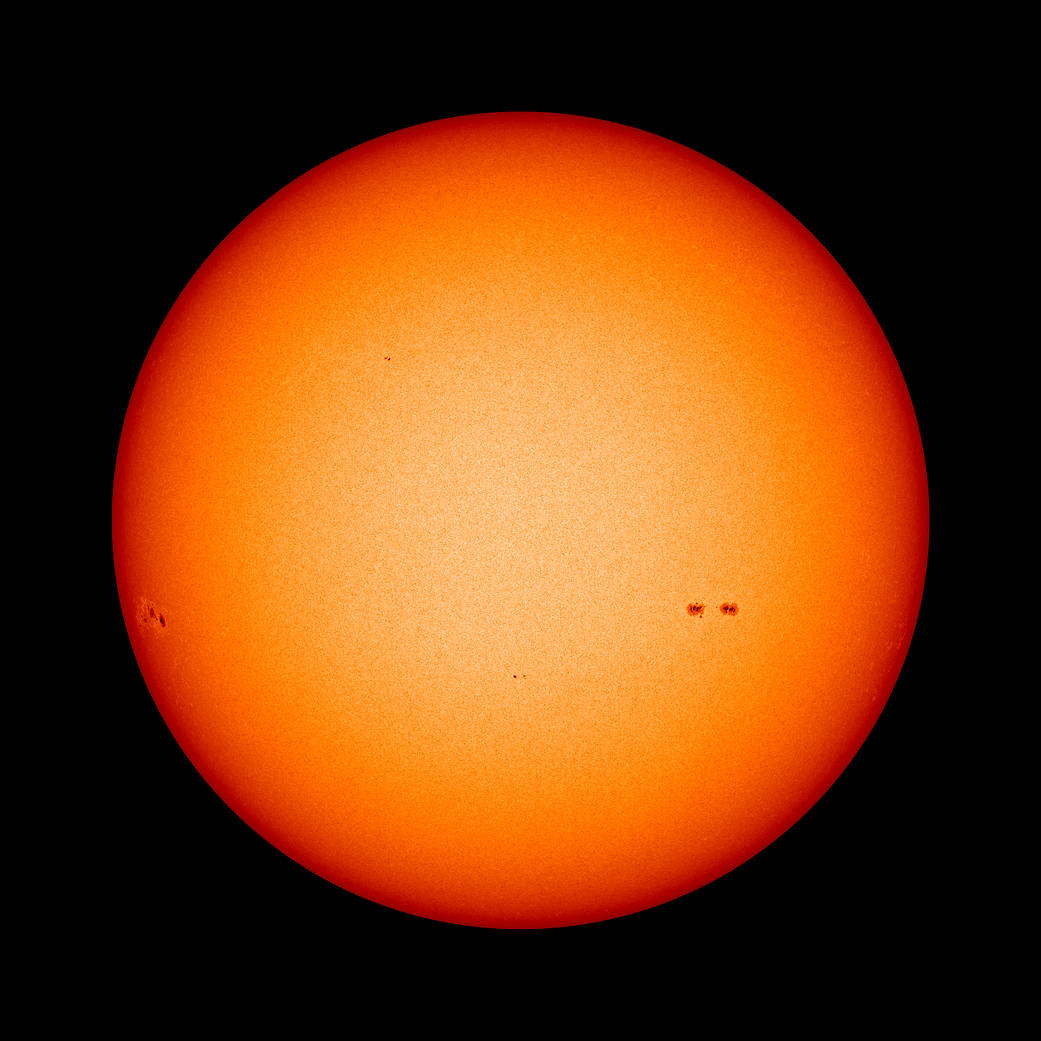
\includegraphics[width=0.75\columnwidth]{limbdark.jpg}
\caption{NASA Solar Dynamics Observatory image of the Sun, showing limb darkening, with the Sun brightest at the centre of the image, due to the line of sight allowing an external observer to see further into the photosphere of the star.}
\label{fig:limb}
\end{figure}
Without limb darkening the star would appear to be uniformly illuminated disk and a transit would appear as a trapezoid, with clear ingress and egress times, allowing for clear measurable transit times. Limb darkening blurs this out into a smooth curve. Figure \ref{fig:limb_model} demonstrates the final impact of limb darkening on transits. If the planet transits the centre of the stellar disk, it is covering the brightest part of the star and so produces the deepest transit. Therefore for the same planet, slightly different observation angles on the transit shadow band see different latitudes of the star transited. This in turn produces different transit depths (and transit durations, due to a smaller chord of the star being transited). The upper panel shows the same system being observed in a narrow range of inclination angles with limb darkening. The lower panels shows the same system without limb darkening. The impact of limb darkening can be mitigated by observing at longer wavelengths (see Figure 3 of \citealt{2007Knutson}).
\begin{figure}[H]
\centering
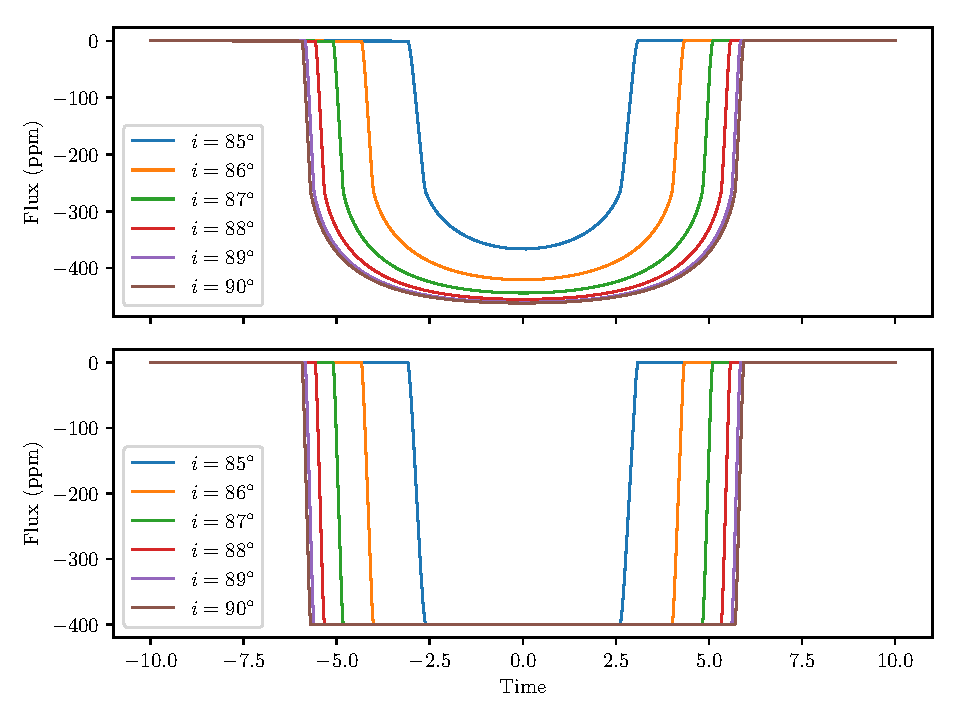
\includegraphics[width=0.75\columnwidth]{limb_d_model}
\caption{Limb darkening blurs trapezoidal transits into curves, and also impacts transit depth, with same system producing a deeper transit when transiting the centre of the stellar disk. At lower inclination angles, a shorter transit is also observed due to the planet transiting a chord of the star smaller than the diameter.}
\label{fig:limb_model}
\end{figure}
Limb darkening must be accounted for when fitting a transit model to observations. Different function forms exists to describe limb darkening, a quadratic form being popular. Many transit model codes either allow for the limb darkening parameters to be included as fixed or free parameters in the fitting procedure, with large tables of limb darkening for various stellar model atmospheres and missions available \citep{2010Sing,2011Claret}.

\subsubsection{Sensitivity to $e$ and $\omega$}
Transit observations also allow constraint on the shape of the orbit, described by the orbital eccentricity $e$  and the argument of periastron $\omega$, the angle between the position of nearest approach and the line of sight. Figure \ref{fig:tran_eccw} shows the impact of varying $\omega$ for a series of model transits. Since for $e>0$ the orbital velocity is no longer constant, the viewing angle of the orbit is now important. If the transit is observed near to periastron then the transit duration will be shorter (due to higher orbital velocity) than for the equivalent $e=0$ orbit (and vice-versa for a transit observed near apastron).
\begin{figure}[H]
\centering
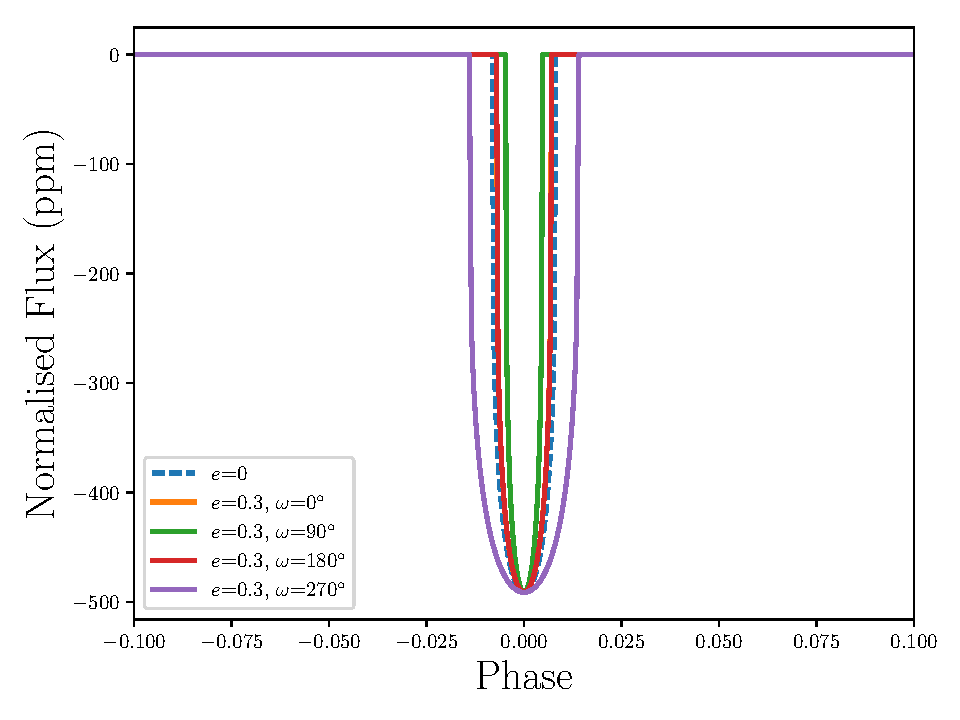
\includegraphics[width=0.75\columnwidth]{eccw}
\caption{The dashed line is the model transit for a circular orbit. The other models are all at an eccentricity of $e=0.3$, with varying $\omega$, between $0^{\circ}$ and $270^{\circ}$. Transits observed near apastron are longer than the circular case, despite the orbit being the same period, due to the lower orbital velocity.}
\label{fig:tran_eccw}
\end{figure}

%As Figure \ref{fig:tran_eccw} shows, transits do exhibit sensitivity to $e$ and $\omega$, however 
\subsection{Estimating stellar density}
A planet transit also gives the opportunity to measure the mean stellar density, derived from Kepler's Third Law and the transit duration, (see \citealt{Winn2010}),
\begin{equation}
\rho_{\star}+k^{3}\rho_{p}=\frac{3\pi}{GP^{2}}\left(\frac{a}{R_{\star}}\right)^{3}.
\label{eq:intro_dens}
\end{equation}
In the above equation, $k=R_{p}/R_{\star}$. This value is typically small and the second term on the left hand side is usually ignored. Therefore, transit photometry allows direct access to the mean stellar density. A caveat on the above equation is the assumption of circular orbits ($e=0$). This is an important result we will return to in Sec \ref{sec:syn} after considering other means of accessing the stellar density in Sec \ref{sec:astero_intro}.

\subsubsection{Biases and shortcomings of method}
As with all forms of observations, large scale transit surveys suffer from biases. For a thorough review, see \cite{2013Gaidos}. If we return to the probability of detecting a transit, Eq \ref{eq:geom}, it is clear that for a fixed stellar radius, orbits on smaller semi-major axes have a higher probability of detection, which biases towards short period planets being detected.  Typically three transits are required to confirm a detection of a planet. While it is possible to observe three transits in only two orbital periods, in most cases this limits any survey to orbital periods $P\leq T/3$ where $T$ is the length of time the survey is in operation. In the case of the 4 year \Kepler mission, that limits detections to orbital periods a little over a year. Eq \ref{eq:tran_dep} shows that a larger planet will have a significantly deeper transit, and so easier to detect. This biases towards giant planets. Additionally the same size planet will produce a much deeper transit around a smaller star. This limits the spectral types of stars that are typically searched for transits, to smaller, cooler stars of FGKM types. This constraint also means the giant stars are not typically included in transit surveys e.g. a 1\Rj transit around a 1\Rs star produces a $>10\e{4}$ppm signal. Around a low luminosity red giant of just $4\Rs$, the transit would be just ${\sim650}$ppm.

Additionally any other signature that induces periodic variations in the lightcurve of a star can be initially identified as a planetary signature, when it is in fact a false positive, or entirely hide the signature of a planet. Sunspots, a surface signature of stellar activity can produce similar brightness variations to that of a small planet. A final problem can be the impact of contaminating light from other stars in the vicinity of the target star. In particular, eclipsing binaries in the background can, when they contribute only a small fraction of the total light of the lightcurve, have the appearance of a transit of the object being imaged. Background eclipsing binaries are the primary source of false positives in \Kepler data \citep{2010Batalha_fp}.

The final shortcoming of the transit method is that it is insensitive to the mass of the planet directly. If the system contains multiple transits in close orbits then variation in the timing of the transits (TTVs) due to dynamical effects can help constrain the masses of the planets \citep{2011Ballard}. 

Normally a second independent detection is required to validate the detection of a planet. Typically this is the ``Doppler wobble'' or radial velocity method, thereby giving constraint on the planet radius and mass separately. However, additional transits of the same depth observed by a different observatory and wavelength are also accepted since transits are achromatic \citep{2015Desert} e.g. Kepler-22b, which was observed by \Kepler and \emph{Spitzer} to confirm it as a planet, as radial velocity observations were unable provide a precise measurement of mass, just an upper limit \citep{2012Borucki}.

\subsection{Dopper wobble}\label{sec:doppler}
In a planetary system, all masses orbit the combined barycentre. For a multi-planet system, such as the Solar System, this is a complicated function of time. For a simple two body system on a circular orbit, the barycentre can be considered a fixed point around which both bodies orbit. 

For systems with 3 or more bodies, the motion of the barycentre is a complicated pattern in space. Given the vast mass difference between stars and planets, the barycentre typically lies inside or near to the star, which will appear to wobble in space due to the influence of any orbiting planets. 

Typically these measurements are taken by comparing the observed spectral lines of a star against a known reference spectrum. The periodic red and blue shifting of the spectrum can be translated into a signal of a planet ``wobbling'' the host star. The size of the wobble induced by a Jupiter mass planet around a Sun-like star on a similar orbit to Jupiter is of the order $10$ms$^{-1}$.  For an Earth analogue i.e, Earth mass planet on a 1 year orbit, that signal is around 0.1ms$^{-1}$. One weakness of this method is that only the component of the wobble along the line of sight can be measured, as such only $M\sin i$ can be measured, unless there is independent constraint on the inclination of the planet. If the system also transits then it can be assumed that $\sin{i}\sim 1$ and so the inferred mass is close to the true mass.
Otherwise the mass estimate is only the minimum possible mass.


For non-circular orbits, the shape of the velocity curve can also give strong constraint on the eccentricity and orientation of the orbit. Figure \ref{fig:rv_model} shows several radial velocity curves for the same hypothetical planet, with the only change being the orbital eccentricity. 
\begin{figure}[H]
\centering
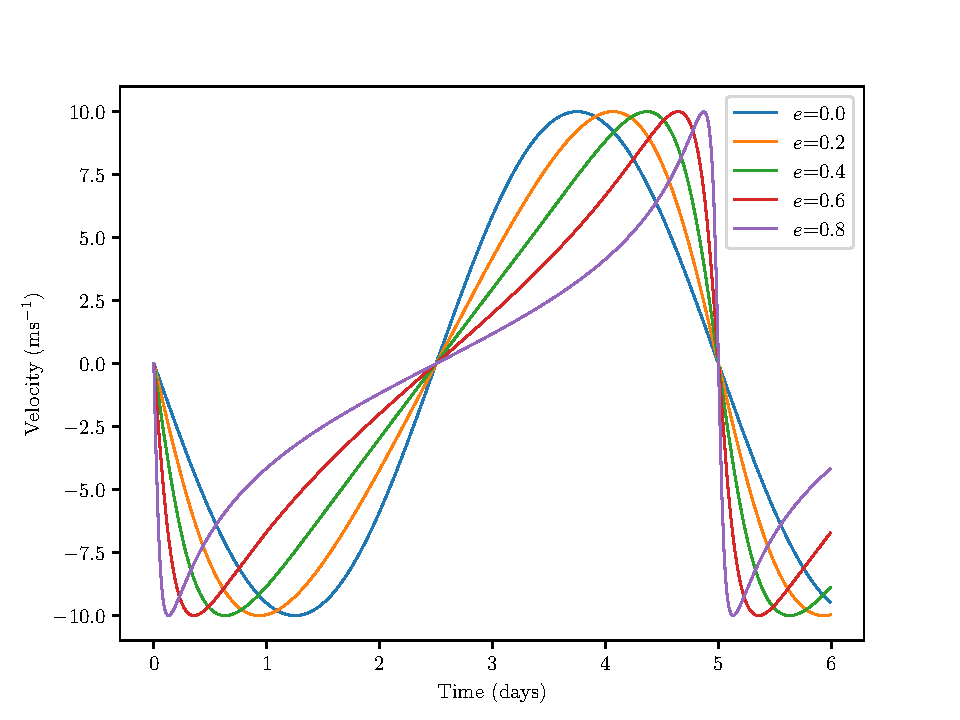
\includegraphics[width=\columnwidth]{RV.pdf}
\caption{Model radial velocity curves for a planet inducing a 10ms$^{-1}$ in its host star, for a variety of orbital eccentricities.}
\label{fig:rv_model}
\end{figure}

The equation governing the observed radial velocity curve of the star is,
\begin{equation}
V(t)=K(\cos{f(t)+\omega} + e\cos{\omega}), 
\label{eq:doppler}
\end{equation}
where $K$ is the semi-amplitude of the wobble, $e$ the orbital eccentricity, and $\omega$ the argument of periastron. $\omega$ is related to the angle between the planet's position  when closest to the star (periastron), and when the orbit crosses the reference plane. $f(t)$ is called the true anomaly, and is a complicated function of time and orbital eccentricity that must be solved numerically for cases where $e>0$. 
For more information see \citet[Ch. 2]{2011Perryman_book}. 

$K$, the semi-amplitude, is related to the mass of planet by the following equation \citet[Eq. 1]{1999Cumming},
\begin{equation}
K=\left(\frac{2\pi G}{P}\right)^{1/3} \frac{M_{P} \sin{i}}{(M_{\star}+M_{P})^{2/3}} \frac{1}{(1-e^2)^{1/2}}.
\label{eq:k_amp}
\end{equation}
It should be clear from this equation that the mass of the planet $M_{P}$ is not directly accessible from the semi-amplitude. However if the approximation is made that $M_{P}\ll M_{\star}$, then the denominator simplifies to $M_{\star}$, and the mass of the planet can be accessed, with only a $\sin{i}$ term remaining, due to the unknown system inclination $i$ with respect to the line of sight. When combined with the transit method, constraint can be placed on all major planetary properties, as $i$ may be inferred from the transit.  
\subsubsection{Biases and shortcomings of method}\label{sec:doppler_probs}
If we consider Eq \ref{eq:k_amp} it is clear that for stars of the same mass either shorter period planets, or higher mass planets will produce the strongest signal. As such the method is biased towards detecting such hot Jupiter type planets. In a reversal of the situation for transits, the radial velocity method is particularly sensitive to the shape of the planet's orbit ($P, e$ and $\omega$), but not to the radius of the planet.

Again stellar activity can have severe effects on the detection of planets, and since the photometric lightcurve may not be available, separating a planetary signal from a stellar rotation induced signal can be extremely difficult, and false positive planets have been reported in literature \citep{2014Robertson}. 

Rapidly rotating stars are also a problem for radial velocity observations, since the star is not resolved, and the spectrum observed is hence some average given by the contributions from across the disc of the star. As such, rapid rotation broadens the spectral line that is being measured. This somewhat limits the typical target selection for Doppler surveys to lower mass stars, which tend to rotate more slowly than their higher mass conunterparts. A final problem with higher mass stars is a lack of spectral lines, due to higher temperatures leading to most elements being highly ionized.  

Typically Doppler surveys target lower main sequence targets (see \cite{2017Butler} and references therein), as with transit surveys. However large scale surveys of giant stars are also possible, due to the slower rotation and cooler temperatures of these stars compared to when they were on the main sequence \citep{2004Setiawan,2007Dollinger,Johnson2007a,2014Lee}. This will be returned to in Chapter \ref{chap:reta}. 

As with all observations, radial velocities measurements are subject to noise. For radial velocities it is known as ``stellar jitter''. This noise can be of astrophysical origin (such as granulation, or oscillations) or instrumental in nature \citep{2005Wright,2010Isaacson}. In the case of lower mass main sequence stars, where convection is driving a stellar magnetic dynamo, signatures of activity are present in the velocity measurements and both stellar flares and sunspots can contribute to the jitter signature \citep{1998Saar,2017Oshagh}. 

For more evolved stars, the dominant noise signature within radial velocity measurements are the stellar oscillations themselves \citep{2007Udry,2008OToole}. For giant stars, the amplitude of these oscillations can reach tens of metres per second \citep{Bedding95}, which can severely impact the types of planets detectable around giant stars. To overcome the impact of jitter on observations, more observations are needed, across a longer baseline encompassing several orbital periods to ensure any detected planetary signal is genuine \citep{Reffert2014}. 


The final shortcoming of the method, already mentioned, is that unlike transits very little information on the inclination of the system can be inferred. The only information available is that the planet has a velocity component along the line of sight, i.e. it does not orbit on the plane of the sky (see discussion of astrometry below). Due to the lack of constraint on inclination, the inferred mass of any planet is a lower limit on the true mass of the planet. This does leave potential for some of the giant planets currently considered planets to in fact be stellar or sub-stellar companions. 

\subsection{Other detection methods}
There are additional methods of detecting exoplanets. If the star is relatively nearby, and the planet on a wide orbit, it is possible to directly resolve the planet, such the multiplanet system HR 8799 \citep{2008Marois,2010Marois}. To do so requires separating the small fraction of light reflected (or emitted) by the planet from the glare of the host star. This can be done using adaptive optics, in conjunction with a coronagraph to physically block the incoming light from the star. 

Another method is astrometric wobble, which can be considered similar to the Doppler wobble, projected onto the plane of the sky. As the planet orbits the host, the star orbits around their combined barycentre, this small motion is detectable, with the current $Gaia$ mission expected to detect several thousand exoplanets via this method \citep{2014Perryman}. The astrometric method measures the motion of the star itself directly, whilst the Doppler method as discussed above, measures the velocity of the star.

\subsection{Characterising exoplanets}
Since both the transit and Doppler detection methods are indirect, they rely on observations of the host star to infer the presence of a planet and as such characterising the planet is fundamentally tied to how well characterised the star is. This is a topic that will be returned to throughout this thesis. Do you want to know the radius of a planet from the transit depth at 5\% precision? You need to know the stellar radius to higher precision than this. Want to claim a detection of a Earth-like planet in the habitable zone of a Sun-like star? You need to know the mass and radius of the host star to high precision. In addition to this, the stellar luminosity would be needed to claim a habitable zone detection. This can be measured either from a precise parallax measurement, or through the stellar effective temperature and radius. Asteroseismology can be used to provide high precision stellar radii and masses, a clear benefit to exoplanetary science and the ability to predict the habitability of the exoplanet. Additional planetary parameters such as albedo, atmospheric composition and rotation would also have an impact on the habitability of a planet. The theme of synergies between asteroseismology and exoplanets will be explored further in Sec \ref{sec:astero_intro}.

\section{Planetary system evolution and destruction}
Star and planet evolution are fundamentally linked. Whilst an exhaustive discussion of planet formation is beyond the scope of this work, we will briefly discuss what effect the evolution of a star will have on any planets orbiting it. A good review is given by \cite{2016Veras} for the evolution of planetary systems after the host star leaves the main sequence. 

\subsection{Orbital migration during subgiant expansion}
A topic we will return to throughout this thesis is that the distribution of stellar and planet properties around evolved stars does not match the distributions of planets around main-sequence stars of similar masses. One possible cause is the destruction/ingestion of planets as the star turns off the main-sequence and begins its evolution into a giant star. A more in depth discussion of stellar evolution is given in Sec \ref{sec:stars}. One theory is as the star evolves into a subgiant, the onset or expansion of surface convection zones leads to angular momentum of the orbiting planet being deposited in the star due to tidal forces, resulting in the in-spiral of the planet \citep{2013Schlaufman}. This theory has particularly been invoked to explain the lack of hot Jupiters seen orbiting evolved stars \citep{2013Schlaufman}. A final theory is that the masses of subgiant and giant stars have been overestimated from spectroscopic properties. This topic is explored in Chapter \ref{chap:reta}.

\subsection{Ingestion during RGB ascent}
At larger orbital separation tidal forces are limited between the star and planet initially, and the star can evolve onto, and up the red giant branch before encountering the planet. Several planets doomed to be ingested by their star have been found by the \Kepler mission \citep{Kepler56,Kepler432}. These planets are expected to be ingested by their hosts in a few tens of millions of years, a relatively short timescale in astronomical terms. We return to this in Chapter \ref{chap:evolvedhosts}

Planet ingestion has also been invoked to explain rapid rotation rates seen in some evolved stars \citep{2008Massarotti,2009Carlberg}, as well as enhanced levels of lithium detected in some giant stars \citep{2002Sandquist,2012Adam}.

In the case of our Solar System, the Earth's fate is uncertain, but is believed to end by being consumed by the evolving Sun \citep{Rybicki2001,earthdeath,2016Veras}. As the Sun evolves into a red giant, consuming Mercury and Venus in the process, it will expand to a maximum radius of ~1.2AU, beyond the Earth's current orbit. Significant mass loss during the ascent of the RGB causes the planets orbits to spiral outwards. While this offers hope for the Earth to survive it would still be inside the solar atmosphere. The increased drag on the Earth, and tidal interactions with the expanded Sun will cause the Earth to spiral into the Sun. Mars is expected to survive. All the outer planets are expected to survive, on expanded orbits, until the end of solar evolution.

As we have seen throughout this section, the evolutionary status of the star has a strong impact on the observability, and indeed, existence of any planetary system. We will now move to look at stellar evolution and characterisation, across the main sequence and post main sequence evolution for stars $M\leq2\Ms$.

